\documentclass[justified]{tufte-book}

%% --- note that the file "tufte-book-local.tex" is also read 

%% --- packages

\usepackage{graphicx}      %% figures
\usepackage{eag_names}     %% journal names
\usepackage{natbib}        %% citations
\usepackage{lipsum}
\usepackage{listings}

\usepackage[Bjornstrup]{fncychap}

\definecolor{gray}{rgb}{0.5,0.5,0.5}
\definecolor{lightgray}{rgb}{0.97,0.97,0.97}
\lstset{language=Python,
  aboveskip=4mm,
  belowskip=4mm,
  showstringspaces=false,
  columns=flexible,
  basicstyle={\footnotesize\ttfamily},
  numbers=none,
  backgroundcolor=\color{lightgray},
  numberstyle=\tiny\color{gray},
  keywordstyle=\color{gray},
  commentstyle=\color{gray},
  stringstyle=\color{gray},
  breaklines=true,
  breakatwhitespace=true,
  tabsize=4
}

%% --- start definitions

\graphicspath{{figures/}}  %% default path for figures

\title{EIS Data Analysis in\\Python}
\author[EIS Team]{EIS Team}

\def\arcsec{\hbox{$^{\prime\prime}$}}
\def\ion#1#2{#1\,{\sc\romannumeral #2}\relax}

%% --- end definitions

\begin{document}

\maketitle
\tableofcontents

%% --- the chapters


\chapter{Introduction}

\newthought{The EUV Imaging Spectrometer} --- EIS\sidenote{EIS is part of the Hinode mission and
  was sponsored by the Japan Aerospace Exploration Agency (JAXA), the United Kingdom Space Agency
  (UKSA), and National Aeronautics and Space Administration (NASA) with contributions from ESA and
  Norway. Hinode was launched on September 22, 2006 at 21:36 UTC from the Uchinoura Space Center in
  Japan and continues to operate.} --- was designed to study the solar atmosphere and answer
fundamental questions on the heating of the solar corona, the origin of the solar wind, and the
release of energy in solar flares. EIS observes two wavelength ranges in the extreme ultraviolet,
171–-212\,\AA\ and 245–-291\,\AA\ with a spectral resolution of about 22\,m\AA\ and a plate scale
of 1\arcsec\ per pixel. Solar images can be made by stepping the slit over a region of the Sun and
taking an exposure at each position. A detailed description of EIS is given in the instrument
paper\cite{Culhane:2007}.

This document describes the basic elements of EIS data analysis using new HDF5 level-1 files and
new routines written in the Python programming language. At the beginning of the Hinode mission the
strategy was to release unprocessed level-0 FITS files and software routines written in IDL for
processing these files into a format that could be used for data analysis. Additionally, all of
the routines for computing ancillary information, such as the offsets of the detectors or the magnitude
of the instrumental broadening, were all written in IDL. Unfortunately, IDL is an expensive,
proprietary language, little used outside of solar physics. Python, in contrast, is a free, open
source language that has grown dramatically in popularity since the launch of Hinode, making it an
obvious choice for future software development.

To accelerate the transition to Python we have created a new level-1 product that contains both the
processed level-1 data and the ancillary information needed for data analysis. The alternative
approach, to port all of the existing IDL software to Python, would be time consuming and create
confusion about which routines are being actively supported during the transition. Distributing
level-1 files removes this problem, but does make the user dependent on the team for reformatting
all of the files as bugs are discovered. Since the mission has been going on for some time now, the
number of bugs is likely to be small.

There are several other design decisions that merit some explanation

\begin{itemize}
  \item The data and header information are stored in separate files. Since the data is large and
    unlikely to change, the time-consuming download of these files should only need to be done
    once. The header file is very small and can be updated easily.
  \item HDF5 is used to store the data. This is a very widely used, high-performance file format
    that is well supported by both IDL and Python. The most attractive feature for this application
    is that data is stored in a self-documenting, directory-like tree structure instead of binary
    table extensions.
  \item The data is processed from raw ``data numbers'' to ``photon events'' or ``counts''. The
    default behavior of \verb+eis_prep+ is to convert to calibrated units. With the HDF5 files
    conversion to absolute units is done using a calibration curve in the header file, and several
    different calibration curves can be considered.
\end{itemize}

The remaining chapters of this document describe the contents of the level-1 files and illustrate
how to use these files for data analysis in Python.


\chapter{Prepping the Data and Writing the HDF5 Files}

The level-0 fits files were prepped using the IDL routine \verb+eis_prep+ available via SolarSoft
\citep{Freeland:1998} and the following options
\begin{verbatim}
  default = 1
  save = 1
  quiet = 1
  retain = 1
  photons = 1
  refill = 0
\end{verbatim}
There are 400,000+ EIS level-0 files at present, but on a multi-core machine using the IDL bridge
all of the files can be prepped in under 24 hours. We have prepped all of the available EIS files
and saved them to standard fits files in the usual way. Some important points
\begin{enumerate}
  
\item[\bf units:] As mentioned previously, the units for the output in these level-1 files is
  ``photon events'' or ``counts.''  This means that the statistical uncertainty can be estimated as
  $\sqrt{N}$. Technically the read noise should be added in, but it becomes significant only at
  very low flux levels (1--2 counts).

\item[\bf retain:] Note that the retain keywords preserves negative values. One of the jobs of
  \verb+eis_prep+ is to remove the pedestal from the CCD readout and any time dependent dark
  current. Since the spectral windows are generally narrow, the estimate of the background can be
  too high and the subtracted intensities of the continuum can be negative. This will be dealt with
  during the fitting.

\item[\bf refill:] The warm pixel problem complicates the fitting of EIS line profiles. As
  discussed in software note \#13 in SSW, interpolating the values of missing pixels appears to
  best reproduce the original data. This option is left off during \verb+eis_prep+ so that the
  level-1 fits file preserves the information on the missing pixels. As discussed below, the
  interpolation (via the refill option) is done during the read and this data is ultimately written
  to the HDF5 file. A mask indicating which pixels have been interpolated needs to be added to the
  HDF5 file.
  
\end{enumerate}
Here is a code snippet related to reading the data by looping over the spectral windows.
\begin{lstlisting}[language=idl]
for iwin=0, nwin-1 do begin
  d = eis_getwindata(eis_level1_filename, iwin, /refill, /quiet)
  eis_level1_data[iwin] = ptr_new(d)
endfor
\end{lstlisting}


\chapter{Reading the HDF5 Level-1 Files}

We assume that the reader is familiar with installing Python packages using either ``pip
install`` or Anaconda. This software has been tested using a default Anaconda stack with Python
version 3.7. In this chapter we will give a very brief overview of how to read the HDF5
files. Subsequent chapters will provide details on specific topics.

This code snippet illustrates how to read the level-1 data from spectral window 7 (containing
\ion{Fe}{12} 195.12\,\AA) in Python. Later in this chapter we'll show how to map a wavelength to a
window number.

\begin{lstlisting}
import h5py
import numpy as np

file_data = 'eis_20190404_131513.data.h5'
file_head = 'eis_20190404_131513.head.h5'

f_data = h5py.File(file_data, 'r')
data = np.array(f_data['level1/win07'])
f_data.close()
\end{lstlisting}
The resulting array is \verb+(512, 87, 24)+. That is, 512 pixels along the slit, 87 steps in the x
direction, and 24 pixels in the dispersion direction.

Information from the header file is read in a similar way. For example,
\begin{lstlisting}
f_head = h5py.File(file_head, 'r')
x_scale, = f_head['pointing/x_scale']
date_obs, = f_head['index/date_obs']
wave = np.array(f_head['wavelength/win07'])
radcal = np.array(f_head['radcal/win07_pre'])
f_head.close()
date_obs = date_obs.decode('utf-8')
\end{lstlisting}
Here \verb+x_scale+ is the number of arcsec per step in the raster. Most EIS rasters take more than
1 arcsec per step, which degrades the spatial resolution but increases the cadence. The variable
\verb+radcal+ is the pre-flight calibration curve for this data window. It includes all of the
factors for converting counts directly to erg cm$^{-2}$ s$^{-1}$ sr$^{-1}$. The \verb+decode+ on
\verb+date_obs+ converts from a byte array to unicode.

We can make a quick image by summing the data in the dispersion direction. The
raster is scaled logarithmically.
\begin{lstlisting}
import matplotlib.pyplot as plt

raster = np.sum(data, axis=2)
range = np.percentile(raster, (1, 99))
range = range[1]*np.array([1.0E-2, 1.0])
scaled = np.clip(raster, range[0], range[1])
scaled = np.log10(raster)

plt.imshow(scaled, origin='lower', aspect=1/x_scale, cmap='gray')
plt.title(date_obs)
plt.show()
\end{lstlisting}
\begin{marginfigure}
  \centerline{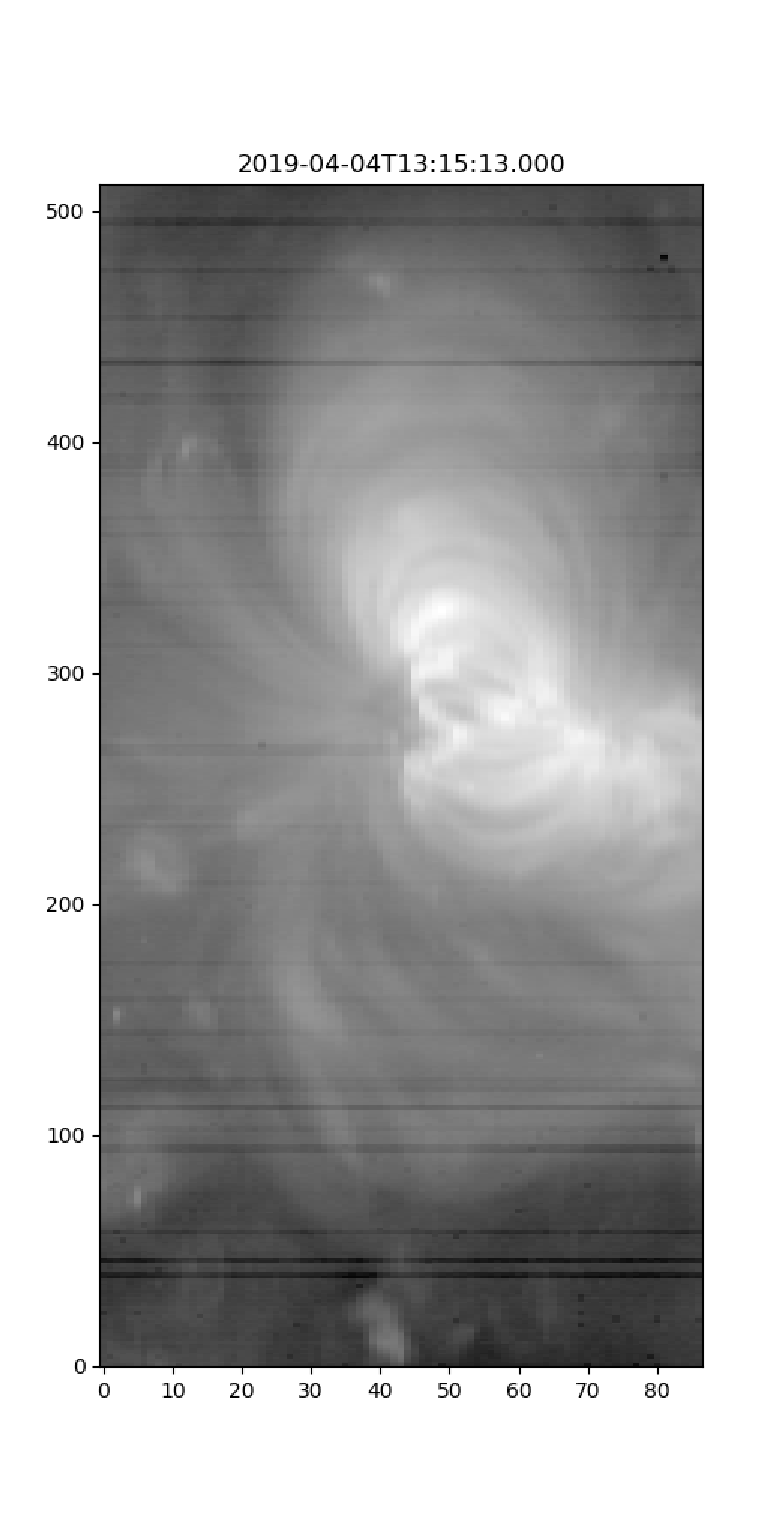
\includegraphics[clip,width=\linewidth]{figures/test_imshow.pdf}}
  \caption{An example image formed by summing the data for the \ion{Fe}{12} spectral window in the
    dispersion direction. In a subsequent chapter we'll discuss fitting the spectra.}
  \label{fig:raster}
\end{marginfigure}

The following code illustrates how to display the spectrum from a single pixel. To convert from
counts to calibrated units we simply multiply by the calibration curve. Note how the array is
addressed differently in Python than in IDL.
\begin{lstlisting}
ix = 48
iy = 326
spec = data[iy, ix, :]
spec_cal = spec*radcal

plt.subplot(1, 2, 1)
plt.plot(wave, spec)
plt.title('units = counts')

plt.subplot(1, 2, 2)
plt.plot(wave, spec_cal)
plt.title('units = ergs cm$^{-2}$ s$^{-1}$ sr$^{-1}$')

plt.show()
\end{lstlisting}
\begin{marginfigure}
  \centerline{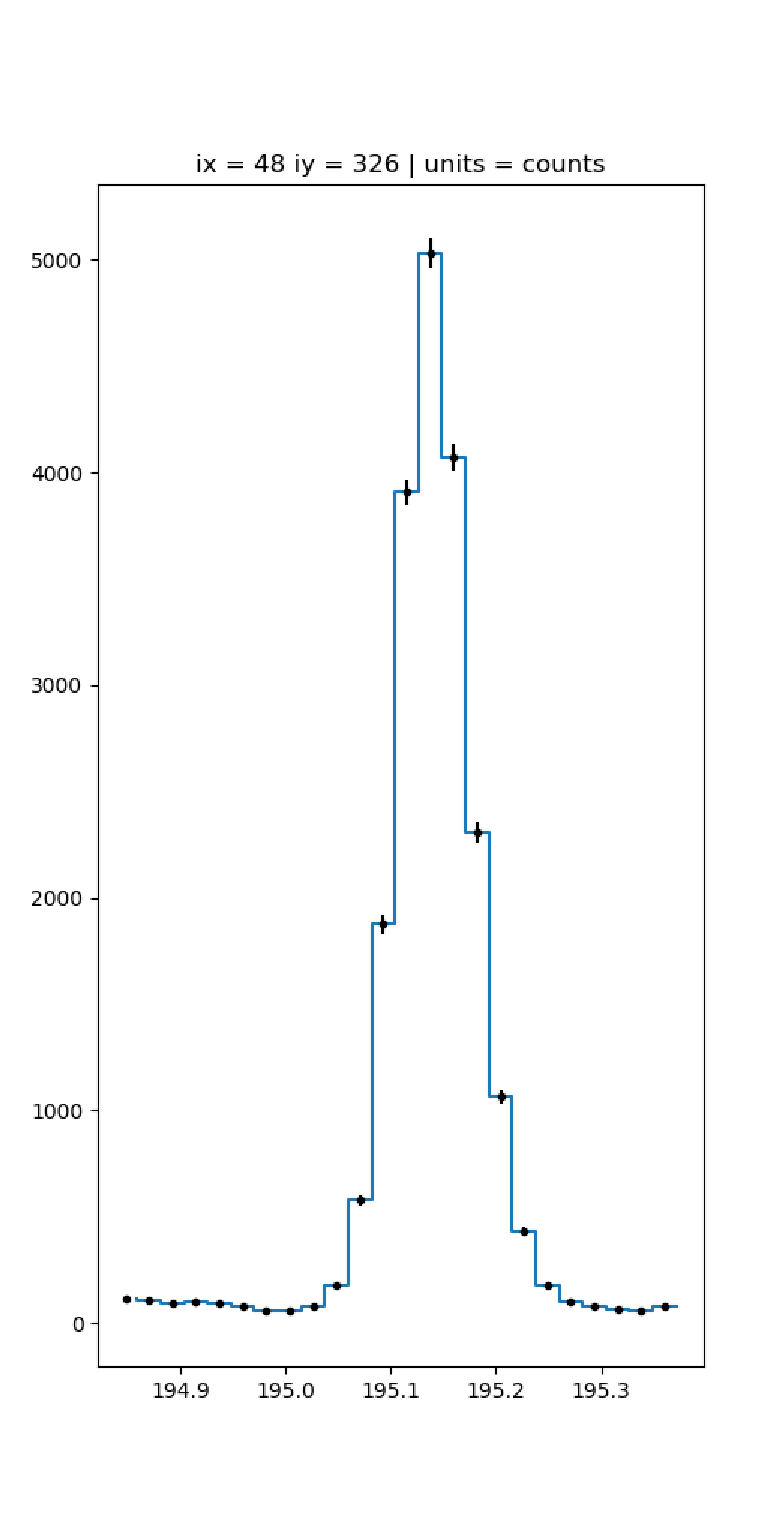
\includegraphics[clip,width=\linewidth]{figures/test_plot.pdf}}
  \caption{An example \ion{Fe}{12} 195.119\,\AA\ line profile from the raster.}
  \label{fig:spectrum}
\end{marginfigure}

We usually don't care about the numbering of the data windows. It's more natural to want to read
the data corresponding to a particularly wavelength. The data in the \verb+wininfo+ group contains
the max and min wavelengths for each data window and allows us to map from wavelength to window
number.
\begin{lstlisting}
f_head = h5py.File(file_head, 'r')
nwin, = f_head['/wininfo/nwin']
dt = np.dtype([('line_id', 'U64'), ('wvl_min', 'f'), ('wvl_max','f')])
wininfo = np.zeros((nwin,), dtype=dt)
wininfo = wininfo.view(np.recarray)
for iwin in range(nwin):
    line_id, = f_head[f'/wininfo/win{iwin:02d}/line_id']
    wvl_min, = f_head[f'/wininfo/win{iwin:02d}/wvl_min']
    wvl_max, = f_head[f'/wininfo/win{iwin:02d}/wvl_max']
    wininfo[iwin].line_id = line_id.decode('utf-8')
    wininfo[iwin].wvl_min = wvl_min
    wininfo[iwin].wvl_max = wvl_max
f_head.close()
\end{lstlisting}
Given a wavelength we can find the window number using the wavelength ranges for each window. Note
that we've converted \verb+wininfo+ to a numpy record array, which behaves similarly to an array of
IDL structures.
\begin{lstlisting}
wvl = 195.119
p = (wininfo.wvl_max - wvl)*(wvl - wininfo.wvl_min)
iwin, = np.where(p >= 0)
\end{lstlisting}
If the result is an empty list, the wavelength is not in the data.

Two final notes on reading the data. First, the contents of the HDF5 files can be displayed using
\verb+h5dump+, which is provided with Anaconda. For example,

\begin{lstlisting}
> h5dump -n eis_20190404_131513.data.h5
FILE_CONTENTS {
group      /
group      /level1
dataset    /level1/intensity_units
dataset    /level1/win00
dataset    /level1/win01
dataset    /level1/win02
dataset    /level1/win03
dataset    /level1/win04
dataset    /level1/win05
. . .
\end{lstlisting}
The actual data associated with each variable can be printed out using the \verb+-d+ option. For
example,
\begin{lstlisting}
> h5dump -d exposure_times/duration eis_20190404_131513.head.h5
HDF5 "eis_20190404_131513.head.h5" {
DATASET "exposure_times/duration" {
   DATATYPE  H5T_IEEE_F32LE
   DATASPACE  SIMPLE { ( 87 ) / ( 87 ) }
   DATA {
   (0): 40.0005, 40.0002, 40.0004, 40.0004, 39.9994, 40.0002, 39.9995, 40,
   (8): 40.0007, 39.9999, 40.0005, 40.0004, 39.9997, 40.0002, 39.9994,
   . . .
}
\end{lstlisting}
Second, there is a Python object \verb+eis_read_raster.py+ that can be used to read the data and head
files. For example,
\begin{lstlisting}
from eis_read_raster import eis_read_raster
filename = 'eis_20190404_131513.data.h5'
wave = 195.119
eis = eis_read_raster(filename, wave)
print(eis.data['index']['date_obs'])
print(eis.data['data'].shape)
\end{lstlisting}
In the chapters that follow we will use the object to do most of the heavy lifting. The routine
\verb+eis_display_window.py+ illustrates how to use the object and matplotlib to click around the
raster and display individual line profiles

\begin{figure}[t]
  \centerline{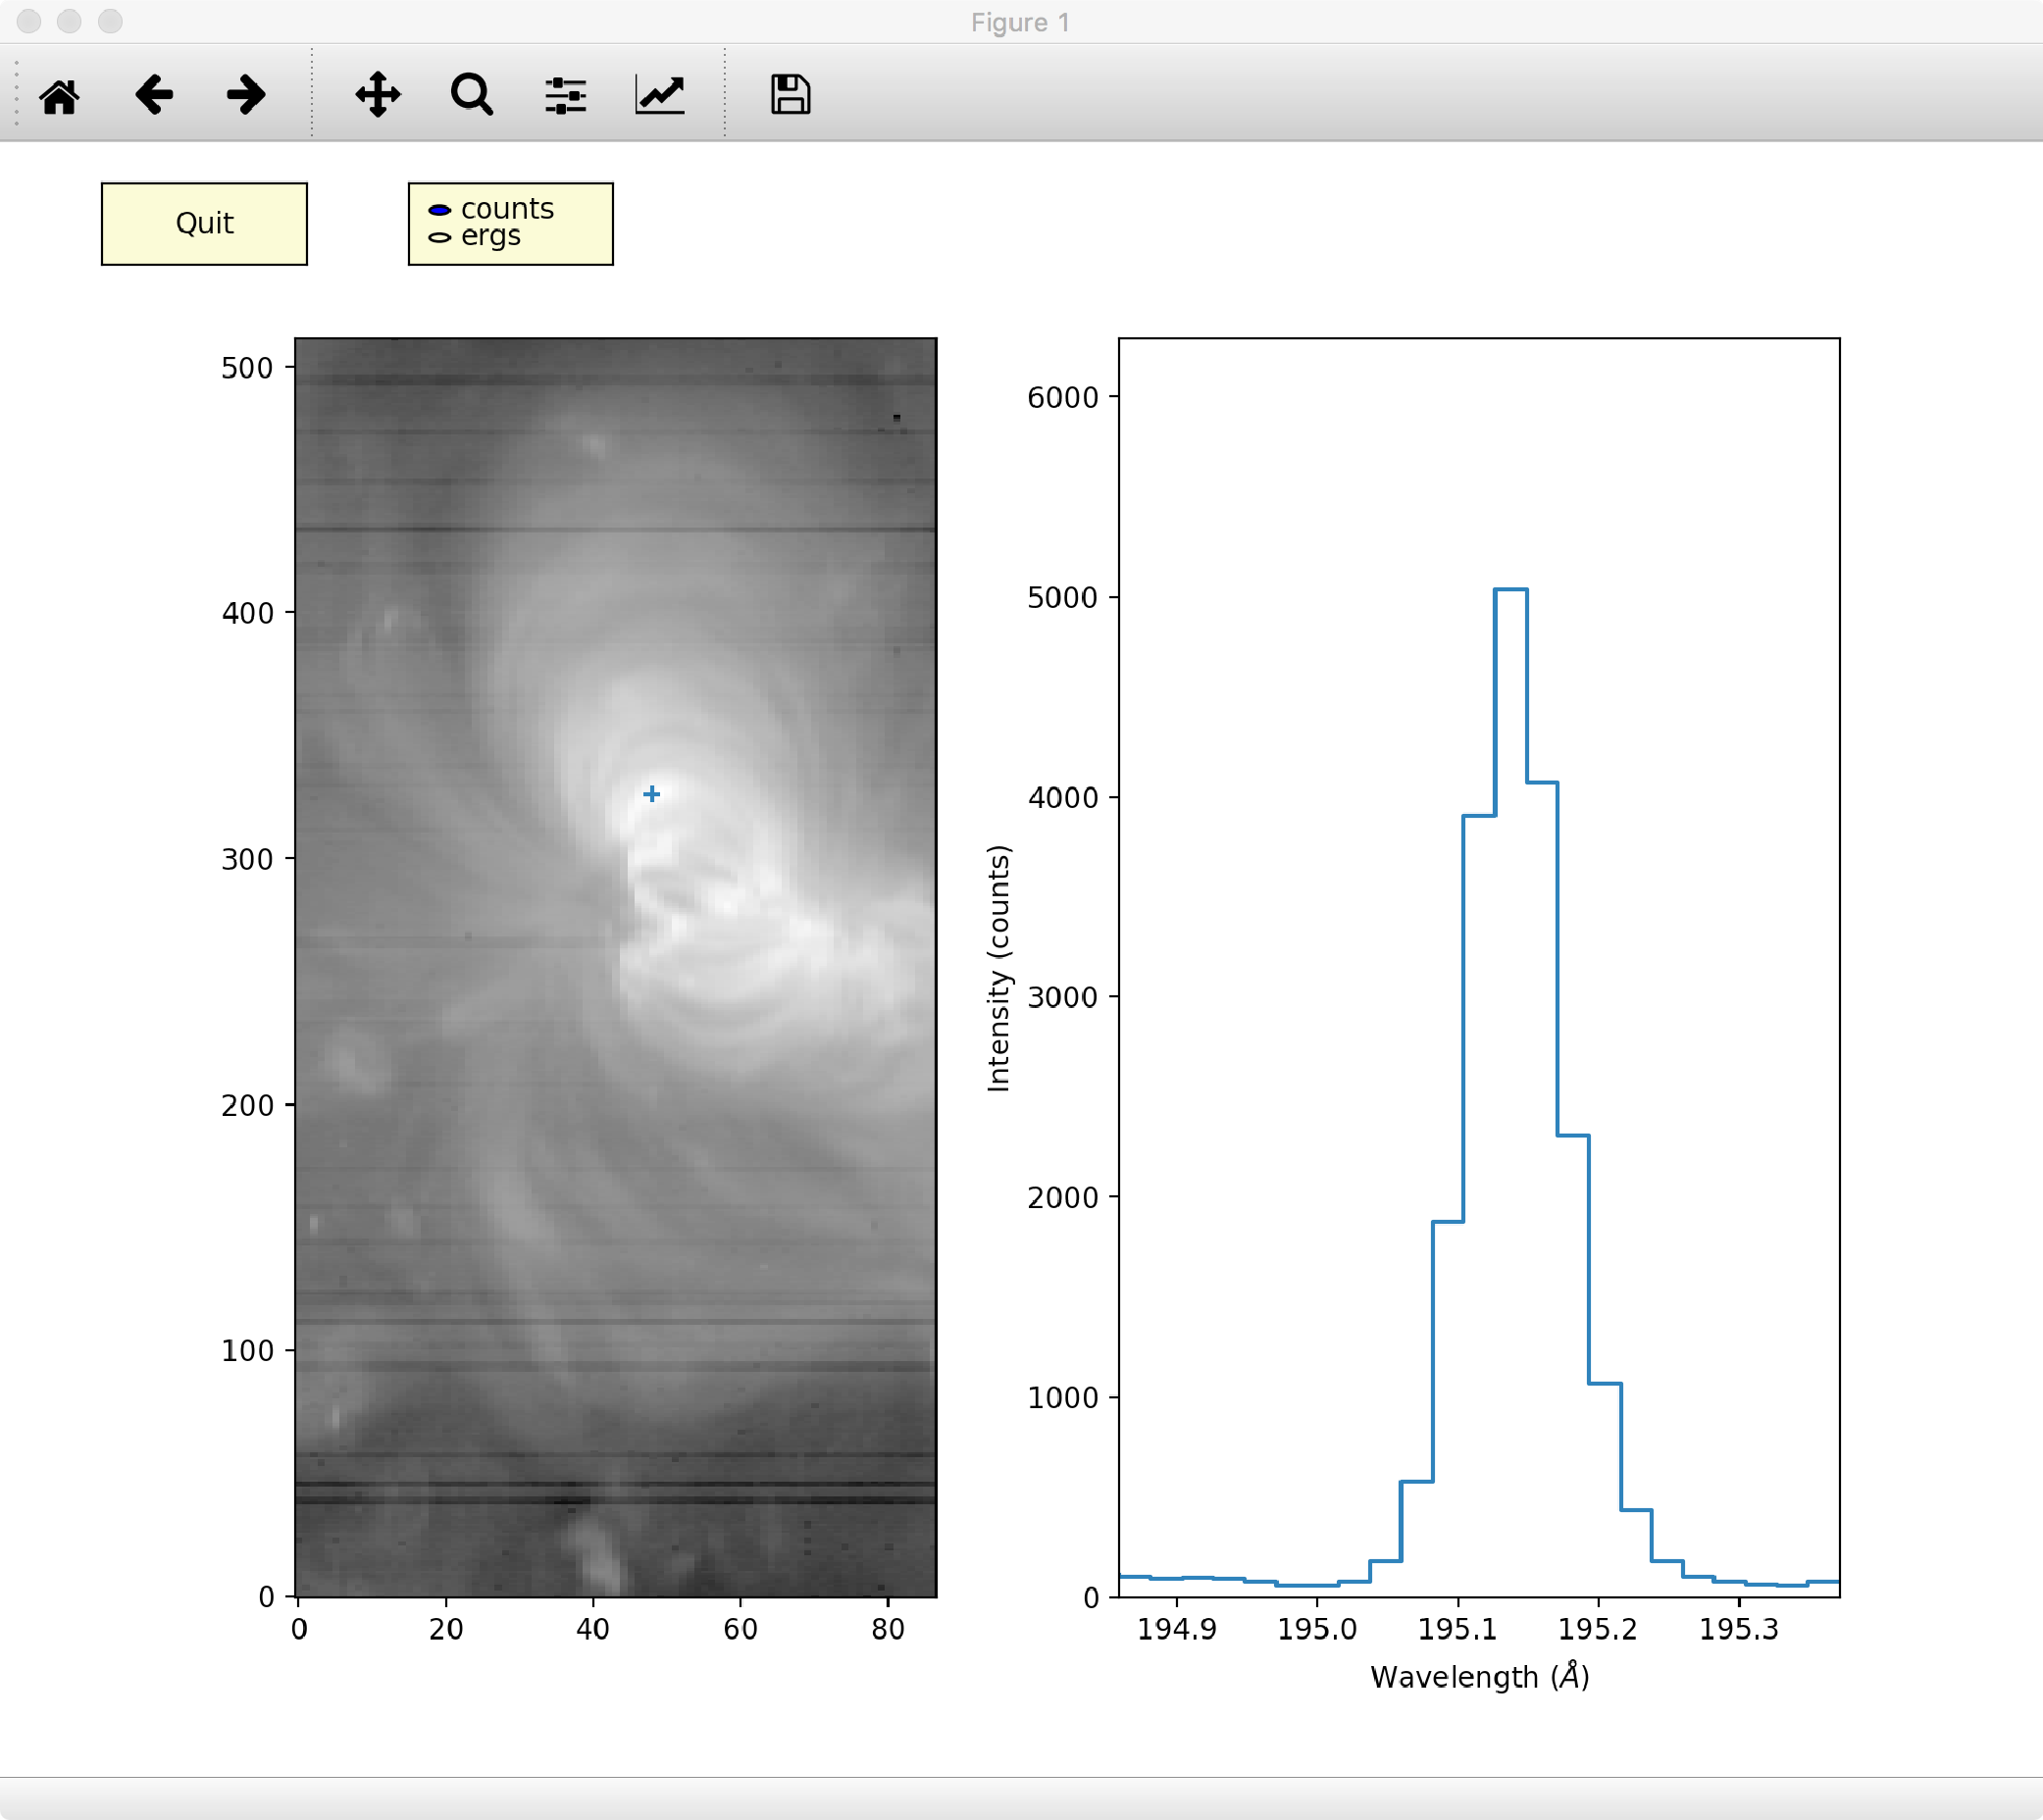
\includegraphics[clip,width=\linewidth]{figures/eis_display_window.pdf}}
  \caption{An example interactive plot showing the raster and the line profile at the selected
    position.}
  \label{fig:matplotlib}
\end{figure}


\chapter{Fitting the Spectra}

Fitting of the spectra involves selecting a spectral line of interest (e.g. \ion{Fe}{12} 195.12\,\AA) from the spectral windows of the data and determining a guess on the fit parameters. The next ingredient for a fit is the selection of an optimization method\sidenote{Here we use a Python implementation of the well-known IDL method mpfit which solves the non-linear least squares problem using the Levenberg-Marquardt algorithm. The Python implementation mpfit.py is found on GitHub (https://github.com/segasai/astrolibpy/) and included in our analysis software.}.

For this we've created a set of fit templates for different spectral lines. An \verb+h5dump+ on the file shows that it contains a \verb+/template+ group for the initial guess on the fit parameters and a \verb+/parinfo+ group containing constraints on the parameters for \verb+mpfit.py+.

\begin{lstlisting}
h5dump -n fe_12_195_119.2c.template.h5
HDF5 "fe_12_195_119.2c.template.h5" {
FILE_CONTENTS {
 group      /
 group      /parinfo
 dataset    /parinfo/fixed
 dataset    /parinfo/limited
 dataset    /parinfo/limits
 dataset    /parinfo/tied
 dataset    /parinfo/value
 group      /template
 dataset    /template/component
 dataset    /template/data_e
 dataset    /template/data_x
 dataset    /template/data_y
 dataset    /template/fit
 dataset    /template/fit_back
 dataset    /template/fit_gauss
 dataset    /template/line_ids
 dataset    /template/n_gauss
 dataset    /template/n_poly
 dataset    /template/order
 dataset    /template/wmax
 dataset    /template/wmin
 }
\end{lstlisting}

 The object \verb+eis_read_template.py+ can be used to read a template file and examine the contents.

\begin{lstlisting}
from eis_read_template import eis_read_template
filename = 'fe_12_195_119.2c.template.h5'
template = eis_read_template(filename)
\end{lstlisting}

This produces the output below, showing the \verb+/parinfo+ group that contains  parameters (peak, centroid, width, background) for a double Gaussian fit along with the parameter constraints. Note that this is specific to using the \verb+mpfit+ method (see the GitHub page for more info).
\begin{lstlisting}
+ template file = fe_12_195_119.2c.template.h5
*PARAMETER CONSTRAINTS*
*              Value      Fixed            Limited                 Limits               Tied
 p[0]     57514.6647          0          1          0       0.0000       0.0000
 p[1]       195.1179          0          1          1     195.0778     195.1581
 p[2]         0.0289          0          1          1       0.0191       0.0510
 p[3]      8013.4013          0          1          0       0.0000       0.0000
 p[4]       195.1779          0          1          1     195.1378     195.2181          p[1]+0.06
 p[5]         0.0289          0          1          1       0.0191       0.0510          p[2]
 p[6]       664.3349          0          0          0       0.0000       0.0000
 \end{lstlisting}

 Next you'll want to prep the data for fitting. Once you've read in a template file, you can use the central wavelength to find the desired spectral window in the data using \verb+eis_read_raster+ as shown in the previous chapter.

\begin{lstlisting}
from eis_read_raster import eis_read_raster
from eis_read_template import eis_read_template

# input data and template files
file_data     = 'eis_20190404_131513.data.h5'
file_template = 'fe_12_195_119.2c.template.h5'

# read fit template
template = eis_read_template(file_template)

# get central wavelength
wmin = template.template['wmin']
wmax = template.template['wmax']
wave = wmin + (wmax-wmin)*0.5

# read raster
raster = eis_read_raster(file_data, wave)
ints   = raster.data['data']
wave   = raster.data['wave']
corr   = raster.data['wave_corr']
\end{lstlisting}

Prepping of the data can be handled at various levels of sophistication at the user's discretion, however, at a minimum it should include handling bad values\sidenote{Negative values are a result of the background subtraction.} in the raster, correcting for the wavelength offsets\sidenote{From thermal drift over the  orbit.}, and computing the errors on the intensities\sidenote{The square root of the counts is a good first-order approximation.}.

\begin{lstlisting}
# get dimensions
ndata = ints.shape
nx    = ndata[0]
ny    = ndata[1]
nz    = ndata[2]

# bad data correction
bad = np.where(ints<0)
ints[bad] = 0.0

# compute error on counts
errs = np.sqrt(ints)

# wavelength correction
newwave = np.zeros(ndata)
for i in range(nx):
    for j in range(ny):
        newwave[i,j,::] = wave-corr[i,j]
wave = newwave
\end{lstlisting}

Now on to the fitting! Now that you have a fit template and the data elements, you can perform a fit of the entire raster by calling \verb+eis_fit_raster.py+\sidenote{Here's what's happening under the hood. The object eis-fit-raster calls eis-scale-guess to scale the initial parameter guess to the data, then calls eis-mpfit to implement the Levenberg-Marquardt fitting. The module eis-fit-deviates contains the callable function that returns the fit deviates computed from a model function for eis-mpfit.}. The fit results can be saved and read back using \verb+eis_save_fit.py+ and \verb+eis_read_fit.py+.

\begin{lstlisting}
from eis_fit_raster import eis_fit_raster
from eis_save_fit import save_fit
from eis_read_fit import read_fit

# fit profile
parinfo  = template.parinfo
template = template.template
fit = eis_fit_raster(wave, ints, errs, template, parinfo)

# save fit output
fit = fit.fit
file_fit = save_fit(fit, file_data)

# read fit output back from file
fit = read_fit(file_fit[0])
\end{lstlisting}

The output fit parameters are stored to a dictionary.

\begin{lstlisting}
background   float64      (512, 87, 1)
centroid     float64      (512, 87, 2)
chi2         float64      (512, 87)
component    int64        1
e_background float64      (512, 87, 1)
e_centroid   float64      (512, 87, 2)
e_int        float64      (512, 87, 2)
e_peak       float64      (512, 87, 2)
e_width      float64      (512, 87, 2)
int          float64      (512, 87, 2)
line_ids     object       (2,)
n_gauss      int16        1
n_poly       int16        1
params       float64      (512, 87, 7)
peak         float64      (512, 87, 2)
perror       float64      (512, 87, 7)
status       float64      (512, 87)
wavelength   float64      (512, 87, 24)
width        float64      (512, 87, 2)
\end{lstlisting}

The above steps are illustrated in the example routine \verb+eis_fit_example.py+, which produces a plot like the one shown below.

\begin{figure}[t]
  \centerline{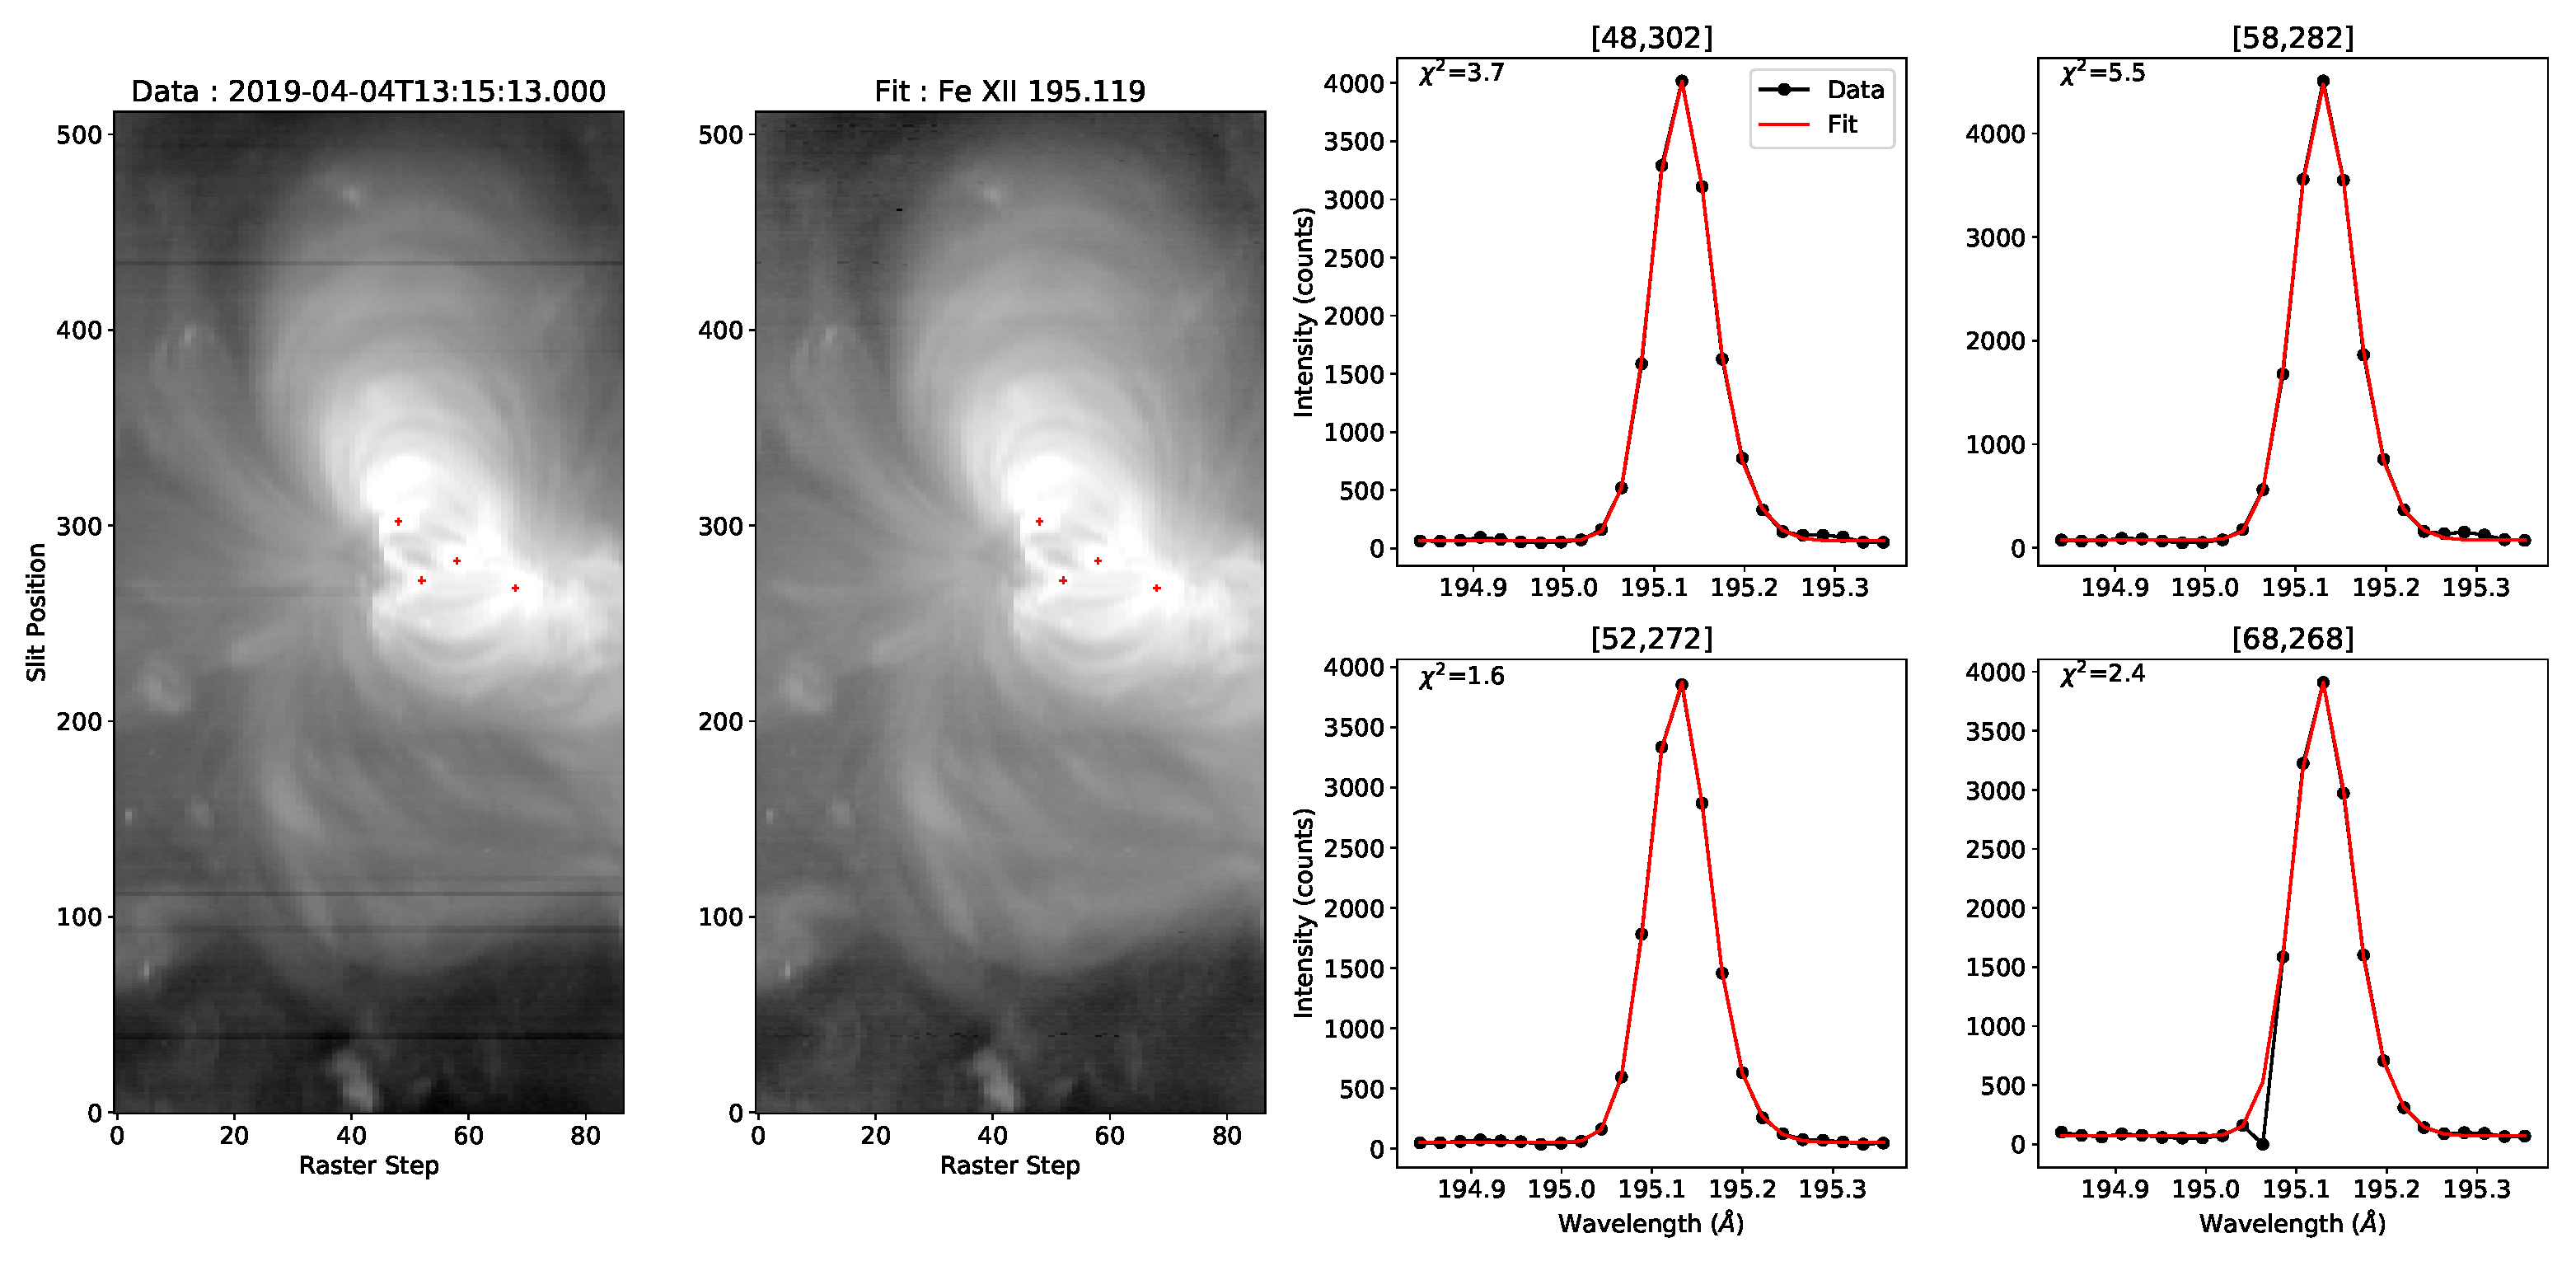
\includegraphics[clip,width=0.8\linewidth,bb=0 0 750 737]{figures/fit_example.pdf}}
  \centerline{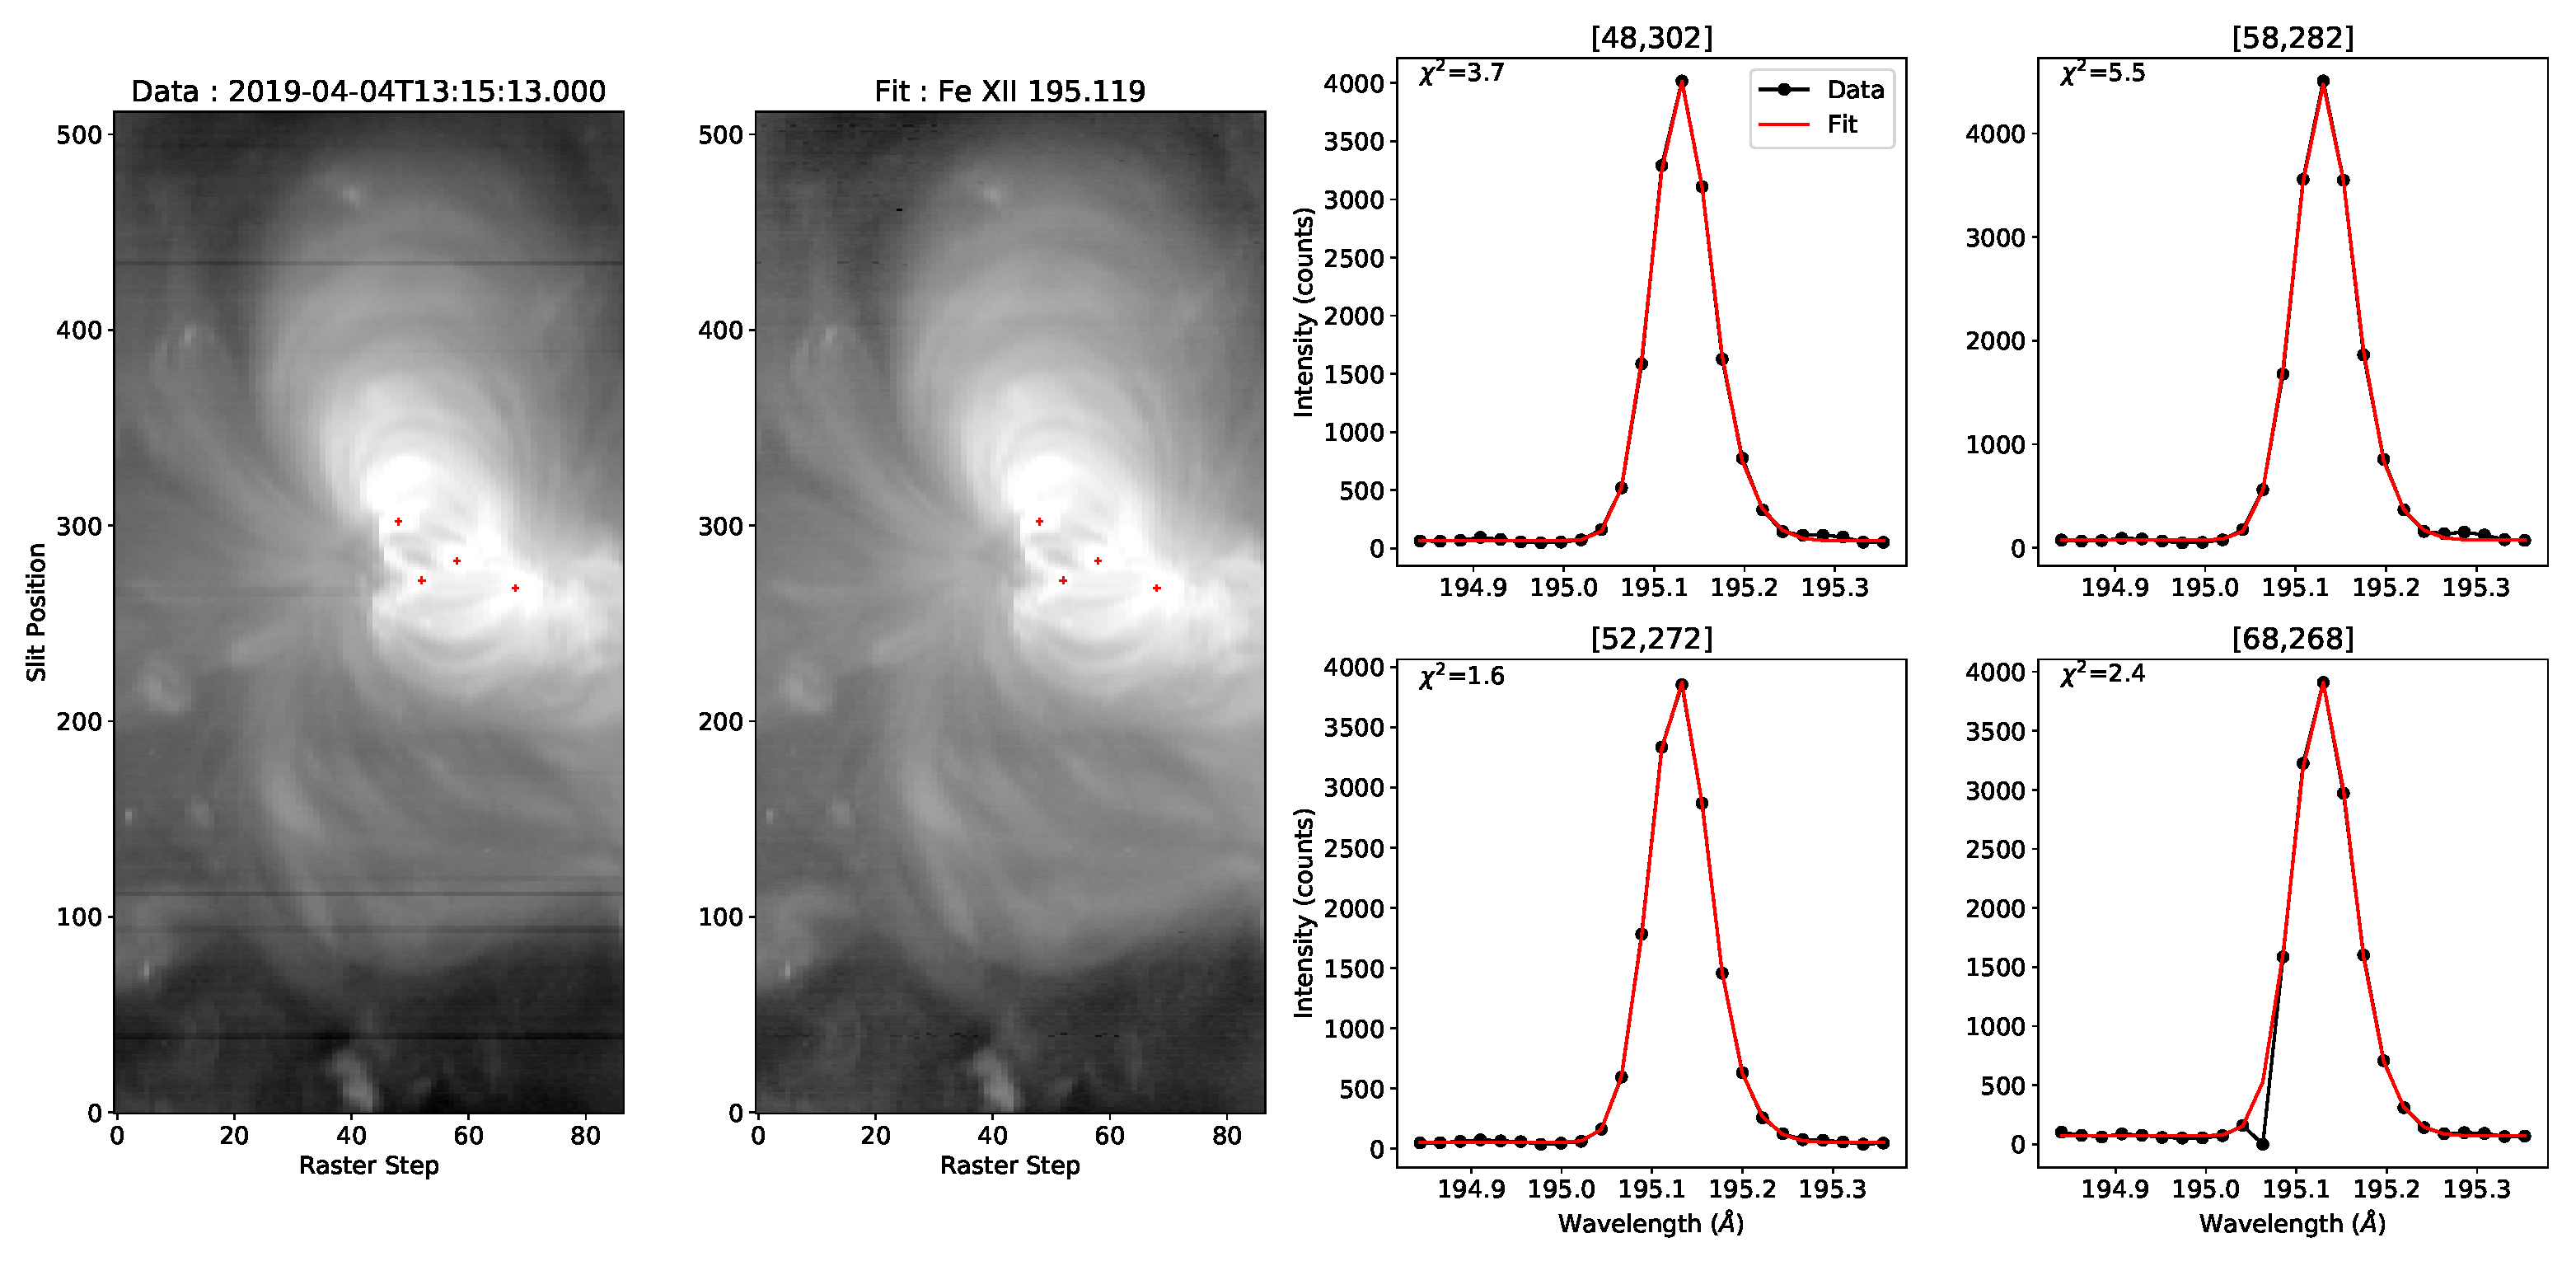
\includegraphics[clip,width=0.8\linewidth,bb=750 0 1500 737]{figures/fit_example.pdf}}  
  \caption{Example line profile fits. The top two panels show the raster formed by summing over the
    profile (left) and fitting each profile (right). The bottom panels show fits to four
    \ion{Fe}{12} 195.119\,\AA\ line profiles.}
  \label{fig:fit_example}
\end{figure}

As a final note about the fitting routines, there's also a parallelized version for fitting the raster that uses the Python Multiprocessing module \sidenote{This uses a pool of processes and parallelizes over the rasters so that each sub-process gets a raster position.}. When using the parallel version, an extra argument can be passed to the function to specify the number of processes to use (default=4) as in the below example. You can also check out the example in \verb+eis_fit_example_parallel.py+.

\begin{lstlisting}
fit = eis_fit_raster_parallel(wave, ints, errs, template, parinfo, ncpu=8)
\end{lstlisting}


\bibliography{eag}
\bibliographystyle{apj}

\end{document}
